\documentclass[a4paper, 12pt]{article}
\usepackage{listings}
\usepackage{xcolor}
\usepackage{graphicx}
\usepackage{float}
\usepackage{amsmath}
\usepackage{amssymb}
\usepackage{amsthm}

\usepackage[
    left=1.0in,
    right=1.0in,
    top=0.75in,
    bottom=0.75in
]{geometry}

\usepackage[
    colorlinks=true,
    linkcolor=blue,	
    urlcolor=blue,
    citecolor=blue
]{hyperref}

\fontsize{9}{11}\selectfont

\lstset{
    language=C++,
	basicstyle=\fontsize{11}{10}\ttfamily\selectfont,
    keywordstyle=\color{blue},
    commentstyle=\color{green!50!black},
    stringstyle=\color{red},
    numbers=left,
    numberstyle=\tiny,
    numbersep=6pt,
    frame=single,
    framesep=2pt,
    framexleftmargin=2em,
    xleftmargin=0pt,
    breaklines=true,
    showstringspaces=false,
    tabsize=4,
    aboveskip=3pt,
    belowskip=3pt
}

\title{\textbf{DS Lab Assignment - 1: Odd 2026}}
\author{Vaibhav Sharma (2501030279)}
\date{August 1, 2026}


\begin{document}
\maketitle

\noindent \textit{All source files here: } \href{https://github.com/Tartuf-57/JIIT-CSE/tree/main/2nd-year/DS/Lab_Assignments/Week_1}{Github Repository}

\bigskip

\noindent\textbf{\large\underline{Answer 1}}
\bigskip
\bigskip
\lstinputlisting[
    language=C++,
]{Q1.cpp}

\begin{figure}[H]
    \centering
    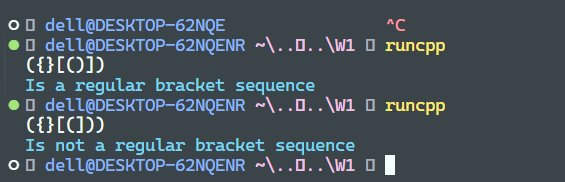
\includegraphics[width=0.7\textwidth]{Q1.png}
    \label{fig:image}
\end{figure}

\newpage

\noindent\textbf{\large\underline{Answer 2}}
\bigskip
\bigskip
\lstinputlisting[
    language=C++,
]{Q2.cpp}

\begin{figure}[H]
    \centering
    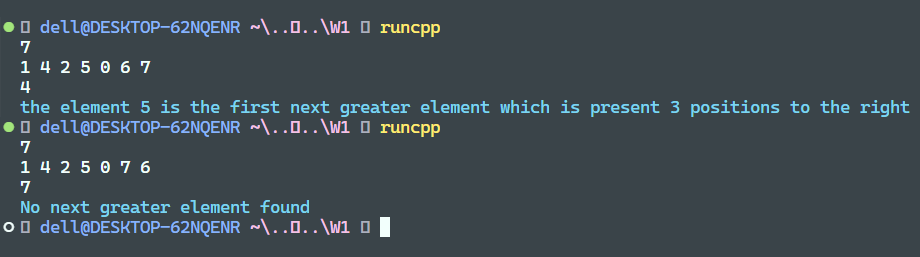
\includegraphics[width=0.9\textwidth]{Q2.png}
    \label{fig:image}
\end{figure}

\bigskip
\bigskip
\bigskip

\noindent\textbf{\large\underline{Answer 3}}
\bigskip
\bigskip
\lstinputlisting[
    language=C++,
]{Q3.cpp}

\begin{figure}[H]
    \centering
    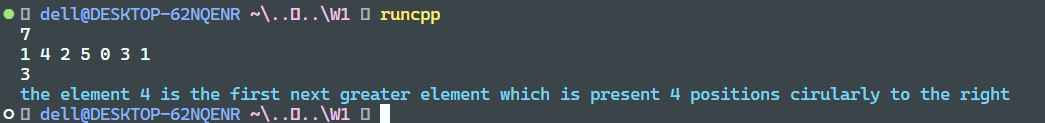
\includegraphics[width=1.0\textwidth]{Q3.png}
    \label{fig:image}
\end{figure}
\bigskip

\noindent\textbf{\large\underline{Answer 4}}
\bigskip
\bigskip
\lstinputlisting[
    language=C++,
]{Q4.cpp}

\begin{figure}[H]
    \centering
    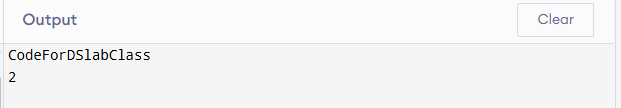
\includegraphics[width=1.0\textwidth]{Q4.png}
    \label{fig:image}
\end{figure}

\bigskip
\noindent\textbf{\large\underline{Answer 5}}
\bigskip
\bigskip
\lstinputlisting[
    language=C++,
]{Q5.cpp}

\begin{figure}[H]
    \centering
    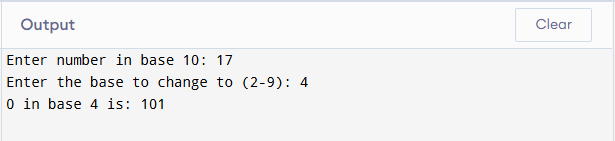
\includegraphics[width=1.0\textwidth]{Q5.png}
    \label{fig:image}
\end{figure}

\bigskip
\bigskip\bigskip
\bigskip

\noindent\textbf{\large\underline{Answer 6}}
\bigskip
\bigskip
\lstinputlisting[
    language=C++,
]{Q6.cpp}

\begin{figure}[H]
    \centering
    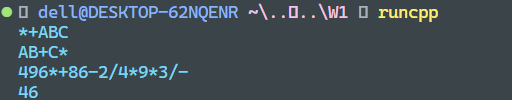
\includegraphics[width=0.7\textwidth]{Q6.png}
    \label{fig:image}
\end{figure}

\bigskip
\bigskip\bigskip
\bigskip
\noindent\textbf{\large\underline{Answer 7}}
\bigskip
\bigskip
\lstinputlisting[
    language=C++,
]{Q7.cpp}

\begin{figure}[H]
    \centering
    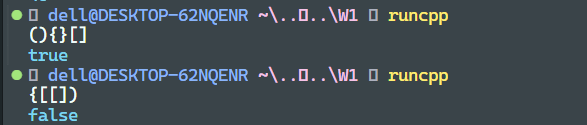
\includegraphics[width=0.7\textwidth]{Q7.png}
    \label{fig:image}
\end{figure}

\bigskip
\bigskip\bigskip
\bigskip
\noindent\textbf{\large\underline{Answer 8}}
\bigskip
\bigskip
\lstinputlisting[
    language=C++,
]{Q8.cpp}

\begin{figure}[H]
    \centering
    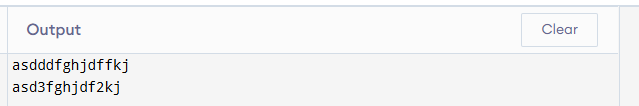
\includegraphics[width=1.0\textwidth]{Q8.png}
    \label{fig:image}
\end{figure}

\noindent\textbf{\large\underline{Answer 9}}
\bigskip
\bigskip
\lstinputlisting[
    language=C++,
]{Q9.cpp}

\begin{figure}[H]
    \centering
    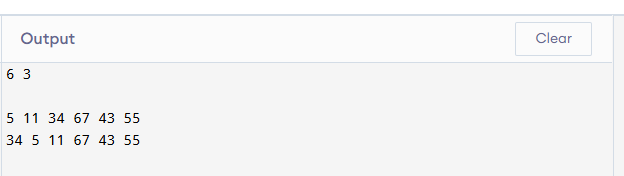
\includegraphics[width=1.0\textwidth]{Q9.png}
    \label{fig:image}
\end{figure}

\noindent\textbf{\large\underline{Answer 10}}
\bigskip
\bigskip
\lstinputlisting[
    language=C++,
]{Q10.cpp}


\begin{figure}[H]
    \centering
    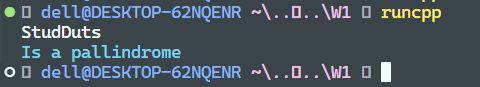
\includegraphics[width=0.7\textwidth]{Q10.png}
    \label{fig:image}
\end{figure}

\bigskip
\bigskip
\noindent\textbf{\large\underline{Answer 11}}
\bigskip
\bigskip
\lstinputlisting[
    language=C++,
]{Q11.cpp}

\begin{figure}[H]
    \centering
    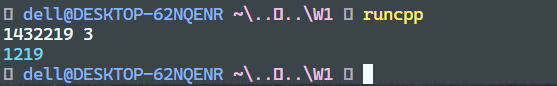
\includegraphics[width=0.7\textwidth]{Q11.png}
    \label{fig:image}
\end{figure}

\bigskip
\bigskip
\noindent\textbf{\large\underline{Answer 12}}
\bigskip
\bigskip
\lstinputlisting[
    language=C++,
]{Q12.cpp}

\begin{figure}[H]
    \centering
    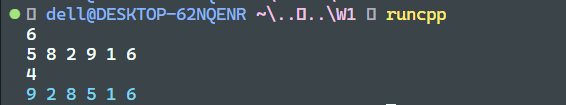
\includegraphics[width=0.7\textwidth]{Q12.png}
    \label{fig:image}
\end{figure}

\bigskip
\bigskip
\noindent\textbf{\large\underline{Answer 13}}
\bigskip
\bigskip
\lstinputlisting[
    language=C++,
]{Q13.cpp}

\begin{figure}[H]
    \centering
    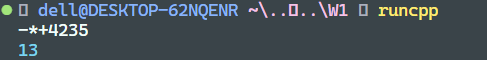
\includegraphics[width=0.7\textwidth]{Q13.png}
    \label{fig:image}
\end{figure}

\end{document}